\section{Wi-fi Protected Access 2 - WPA2}

\ac{WPA}2 is a security protocol developed by Wi-fi Alliance. Officially released in 2004 by \ac{IEEE}802.11i \cite{4248378}, \ac{WPA}2 immediately superseded \ac{WPA} in 2006. Up until now, \ac{WPA}2 is extolled to be stable and safe in wireless environment. In comparison with \ac{WEP} and \ac{WPA}, \ac{WPA}2 is a great leap forward of \ac{WLAN} security. First, it uses \ac{AES} encryption algorithm, which is much stronger than\ac{RC4}, to encrypt data. The use of this algorithm provides confidentiality to end users devices or \ac{AP}s. Second, the complexity of \ac{CCMP} makes the brute force attack impossible \cite{alblwi2017survey}.
\subsection{AES}
\ac{AES} is an encryption algorithm established by \ac{NIST} in 2001 \cite{standard2001announcing}. The core of \ac{AES} is Rijndeal algorithm which is developed by Vincent et.al in \cite{daemen1999aes}. It is the most reliable block cipher till to date. As a result, \ac{AES} has officially superseded \ac{RC4} in \ac{WEP} or \ac{WPA} for \ac{WLAN} encryption algorithm. Up until now, there is no recorded successful attack to break the key of \ac{AES} encryption. The details of algorithm is described in \cite{daemen1999aes}.
\subsection{CCMP}
The combination between \ac{AES} and a complex cryptographic protocol would result in \ac{CCMP}. This protocol consists of two sub-protocols. The first one is Counter Mode \ac{AES} for providing encryption. The second one is \ac{CBC-MAC} for providing authentication and data integrity. Due to $128bits$ key block cipher property, \ac{CCMP} is strongly resistant to several attack techniques. As a result, \ac{WPA}2 employs \ac{CCMP} encryption technique to alleviate the vulnerabilities of \ac{WEP} and \ac{WPA} so that it would attain confidentiality, authentication and access control.
\subsection{General AES-CCMP mechanism}
\ac{AES}-\ac{CCMP} in \ac{WPA}2 encryption undergoes 4 main steps \cite{kolokithas2015hacking}:
\begin{steps}
	\item Construct \ac{CCMP} by using $48bits$ replay protection \ac{IV} and keyID.
	\item Compute \ac{MIC} by using \ac{CCMP} header, session key and plaintext.
	\item Generate the nonce by using \ac{IV} and plaintext
	\item Get ciphertext through encrypting plaintext, session key, \ac{MIC}, nonce and the CCMP header achieved from previous step.
\end{steps}

The details of the algorithm are described in \autoref{fig:ccmp}% cite hinh vao%

\begin{figure}
	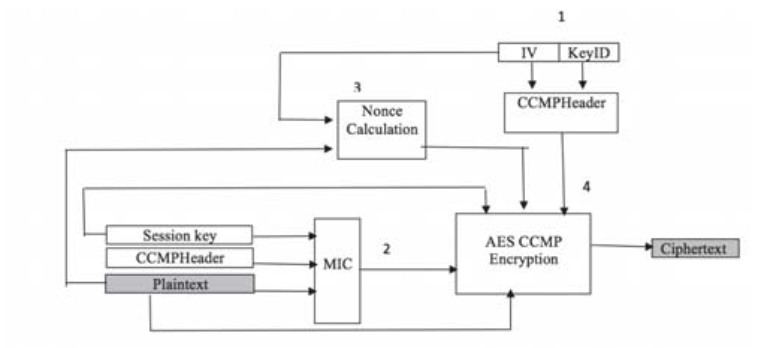
\includegraphics[scale=0.3]{images/ccmp.png}
	\caption{AES-CCMP operation}
	\label{fig:ccmp}
\end{figure}

\subsection{WPA2 advantages}
The \ac{WPA}2 has several amelioration over \ac{WEP} and \ac{WPA} as it alleviates all vulnerabilities in those previous security protocols. 

The biggest improvement of \ac{WPA}2 is the employment of \ac{AES} algorithm. This algorithm demands 2120 operations to break through the key. As recording, there is no successful attack on \ac{WPA}2 until to this moment.% Cite tai lieu%

Another improvement is the data integrity is provided not only for the data but also for the packet header as well. This leads to the outrage security in \ac{WLAN}.

The length of \ac{WPA}2, which is $48bits$, to avoid the \ac{IV} collision and keystream reuse attack. Furthermore, if the $128 bits$ shared key is obtained, the attacker will take several minutes to several weeks to break the encryption which is contingent to the complexity of the user password. The password length is ranged from $8$ to $93$ characters, there are $95^8 \rightarrow 95^{93}$ combinations of user passwords that negates all brute force effort %cite tai lieu%

\ac{WPA}2 is not only the most secure protocol but a light-weighted protocol as well. It adds two nuances for fast roaming. They are PMK caching and pre-authentication support. As a result, timing sensitive applications such as VoIP and videos can be transmitted smoothly over network. Another network performance nuance is cost-balance, manageability and risk mitigation between user authentication and server authentication by defining 802.1x/\ac{EAP} for mutual authentication.

\subsection{WPA2 vulnerabilities}

In spite of great leap forward in security, \ac{WPA}2 can be exposed to several attack techniques such as \ac{Dos} attack, Brute force attack, man-in-the-middle attack and \ac{GTK} attack \cite{alblwi2017survey}.



